%-------------------------------------------------------------------------------
% 请勿删除本注释
% Free Response Question 2
%
% 指引:
% 如在小问之前有通用问题描述,请放置于此
%-------------------------------------------------------------------------------
\begin{figure}[H]
\centering
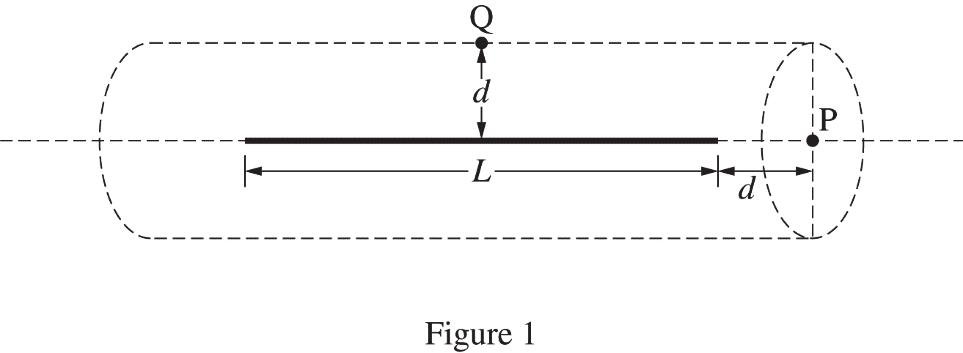
\includegraphics[scale=0.3]{images/img-022-035.png}
\end{figure}


\question
A thin wire of length $L$ has a uniform charge density $+\lambda$. A cylindrical Gaussian surface of radius $d$ is drawn with the wire along its central axis, as shown above. Point $P$ is located at the center of one end of the cylinder, a distance $d$ from the end of the wire. Point $\mathrm{Q}$ is on the edge of the cylinder directly above the center of the wire, as shown above.

A student says, "Gauss's law can be used to find the electric flux $\Phi$ through the Gaussian surface." % 请删除并替换本行,与上一行 \question 之间不要留空行

\begin{parts}

%-------------------------------------------------------------------------------
% 请勿删除本注释
% Part (a)
%
% 指引:
% 如在小问之前有通用问题描述,请放置于此
%-------------------------------------------------------------------------------

\part
Is the student's statement correct or incorrect?

\underline{\qquad}Correct \qquad \underline{\qquad}Incorrect

If you have chosen "Correct," use Gauss's law to find the electric flux $\Phi$ through the Gaussian surface.

If you have chosen "Incorrect," explain why the student's reasoning is incorrect and why Gauss's law cannot be applied in this situation. % 请删除并替换本行,与上一行 \part 之间不要留空行

%-------------------------------------------------------------------------------
% 请勿删除本注释
% Part (b)
%
% 指引:
% 如在小问之前有通用问题描述,请放置于此
%-------------------------------------------------------------------------------

\part
Two students discuss whether or not they can use Gauss's law to find the electric field at points P and Q. At which of the points, if either, is Gauss's law a useful method for finding the electric field?

\underline{\qquad}At point $P$ only \hspace{2.2cm} \underline{\qquad}At point $Q$ only

\underline{\qquad}At both points $P$ and $Q$ \qquad \underline{\qquad}At neither point $\mathrm{P}$ nor point $\mathrm{Q}$

Justify your answer. % 请删除并替换本行,与上一行 \part 之间不要留空行

%-------------------------------------------------------------------------------
% 请勿删除本注释
% Part (c)
%
% 指引:
% 如在小问之前有通用问题描述,请放置于此
%-------------------------------------------------------------------------------

\part
Assuming the electric potential is zero at infinity, show that the value for the electric potential at point $P$ is given by the following expression. % 请删除并替换本行,与上一行 \part 之间不要留空行
$$
V=\frac{\lambda}{4 \pi \varepsilon_{0}} \ln \left(\frac{L+d}{d}\right)
$$

%-------------------------------------------------------------------------------
% 请勿删除本注释
% Part (d)
%
% 指引:
% 如在小问之前有通用问题描述,请放置于此
%-------------------------------------------------------------------------------
\begin{figure}[H]
\centering
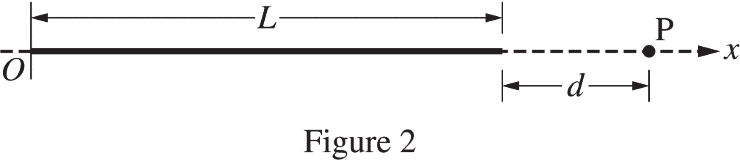
\includegraphics[scale=0.3]{images/img-023-036.png}
\end{figure}

The wire is aligned along the $x$-axis with the origin at the left end of the wire, as shown in Figure 2 above.

\part
A positively charged particle of charge $+e$ and mass $m$ is released from rest at point P. On the axes below, sketch the kinetic energy $K$ of the particle, the potential energy $U$ of the wire-particle system, and the total energy $E_{\text {tot }}$ of the wire-particle system as functions of the particle's position $x$. Clearly label each sketch with $K, U$, and $E_{\mathrm{tot}}$. Explicitly label any maximum with numerical values or algebraic expressions, as appropriate. % 请删除并替换本行,与上一行 \part 之间不要留空行

\begin{figure}[H]
\centering
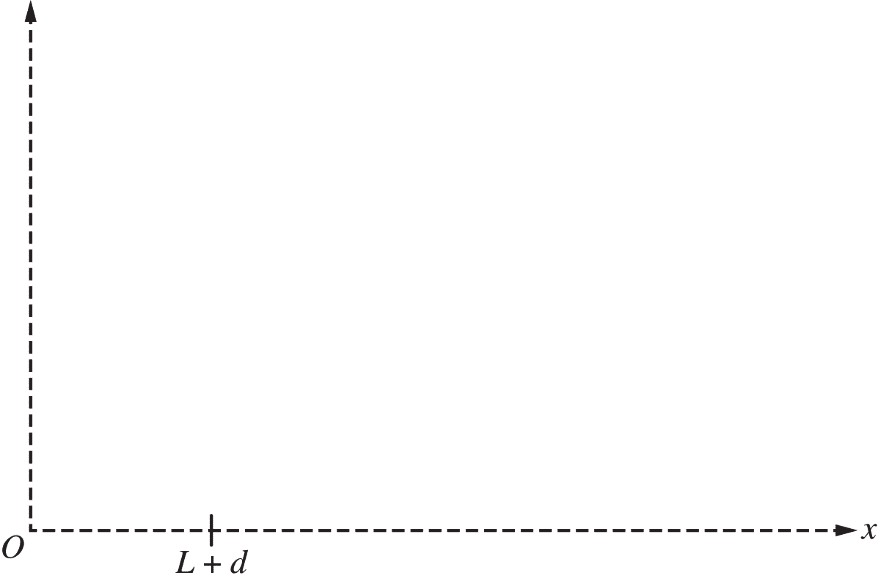
\includegraphics[scale=0.3]{images/img-023-037.png}
\end{figure}

%-------------------------------------------------------------------------------
% 请勿删除本注释
% Part (e)
%
% 指引:
% 如在小问之前有通用问题描述,请放置于此
%-------------------------------------------------------------------------------

\begin{figure}[H]
\centering
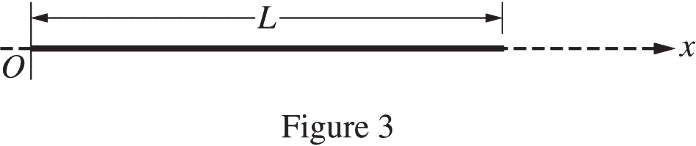
\includegraphics[scale=0.3]{images/img-024-038.png}
\end{figure}

\part
Derive an expression for the magnitude of the electric field due to the wire as a function of the position along the $x$-axis, where $x>L$. Express your answer in terms of $x, L, \lambda$, and physical constants, as appropriate. % 请删除并替换本行,与上一行 \part 之间不要留空行

\end{parts}


